\textbf{Ejemplo 5}\\
Se plantea la construcción de un puente y se han presentado dos proyectos, el primero es un puente colgante a un costo de 850 millones COP y, cada año habrá que darle mantenimiento a la plataforma de asfalto a un costo de 3 millones COP; se estima que las reparaciones serán cada vez mayores y que éstas aumentarán de precio en 2 millones COP cada año, además, cada 5 años habrá que cambiar los cables que sostienen el puente y su costo será de 100 millones COP y, no se prevé que éste valor vaya a cambiar. La segunda alternativa es un puente en concreto a un costo de 900 millones COP y, cada 3 años habrá que reacondicionar las bases a un costo fijo de 25 millones COP; el costo anual de mantenimiento se puede considerar fijo en 5 millones COP. Con una tasa del 25\%, determinar la mejor alternativa.\\


%%%%%%%%%%%%%%%%%%% EJERCICIO 5 %%%%%%

%\newpage %USAR SOLO SI EL SOLUCION QUEDA SOLO Y ES NECESARIO BAJARLO A LA SIGUIENTE PAGINA
\textbf{Solución.}\\
%La tabla ira centrada
\begin{center}
	\renewcommand{\arraystretch}{1.5}% Margenes de las celdas
	%Creacion de la cuadricula de 3 columnas \end{flushleft}
	\begin{longtable}[H]{|C{0.5\linewidth}|C{0.5\linewidth}|}
		%Creamos una linea horizontal
		\hline
		%%%%%%%%%% INICIO TITULO
        %%%%% INICIO FLUJO DE CAJA
		\rowcolor[HTML]{FFB183}
		\multicolumn{2}{|c|}{\cellcolor[HTML]{FFB183}\textbf{1. Asignación periodo focal}}   \\ \hline
		\multicolumn{2}{|c|} {$pf = 0 pav$} \\ \hline
		%%%%%%%%%% FIN TITULO
		%Lo que se hace aqui es mezclar las 3 columnas en una sola
		\multicolumn{2}{|c|}{\cellcolor[HTML]{FFB183}\textbf{2. Declaración de variables}}   \\ \hline
		%%%%%%%%%% FIN TITULO
		%%%%%%%%%% INICIO DE MATEMATICAS
		%Cada & hace referencia al paso de la siguiente columna
		Puente colgante & Puente en concreto \\ 
		i$_{1}$= 0.25 pav & i$_{1}$= 0.25 pav\\
		i$_{2}$= ? pav & i$_{2}$= ? pav\\ \hline
		%%%%%%%%%% FIN DE MATEMATICAS
		%%%%% FIN DECLARACION DE VARIABLES

  		%%%%% INICIO DECLARACION FORMULAS
  
		%%%%%%%%%%% INICIO TITULO
		\rowcolor[HTML]{FFB183}
		\multicolumn{2}{|c|}{\cellcolor[HTML]{FFB183}\textbf{3. Diagrama de flujo de caja}} \\ \hline
		%Mezclamos 3 columnas y ponermos el dibujo
		%%%%%%%%%%%%% INSERCION DE LA IMAGEN
		%Deberan descargar las imagenes respectivas del drive y pegarlas en la carpeta
		%n_capitulo/img/ejemplos/1/capitulo1ejemplo1.pdf  (el /1/ es el numero del ejemplo)
		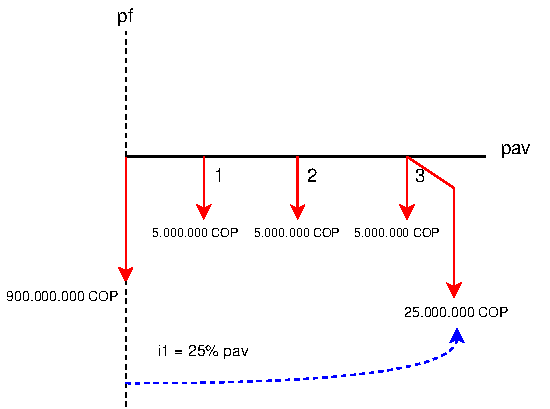
\includegraphics[trim=-5 -5 -5 -5 , scale=1,width=150px, height=125px]{9_Capitulo/ejemplos/6/Capitulo9Ejercicio6a.pdf} &  
		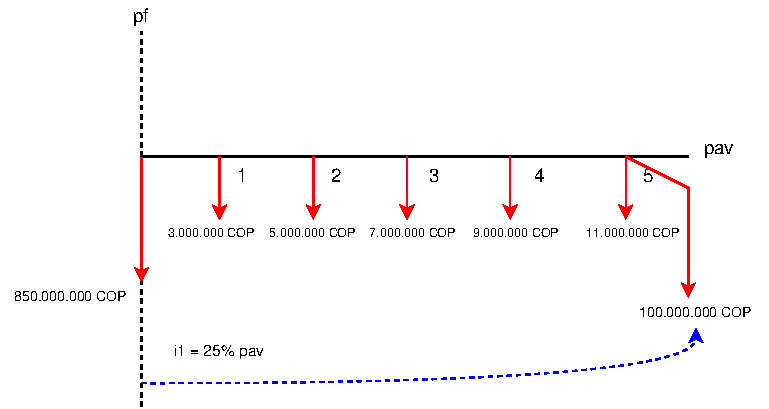
\includegraphics[trim=-5 -5 -5 -5 , scale=1,width=175px, height=125px]{9_Capitulo/ejemplos/6/Capitulo9Ejercicio6b.pdf}  \\ \hline
		%%%%%%%%%%%%% FIN INSERCION DE IMAGEN
		%%%%%FIN FLUJO DE CAJA



		%%%%% INICIO DECLARACION FORMULAS
		%%%%%%%%%%% INICIO TITULO
		\rowcolor[HTML]{FFB183}
		\multicolumn{2}{|c|}{\cellcolor[HTML]{FFB183}\textbf{4. Declaración de fórmulas}}    \\ \hline
		%%%%%%%%%%% FIN TITULO
		%%%%%%%%%%% INICIO MATEMATICAS
		\multicolumn{2}{|c|}{$\sum F_{n}(1+i)^{-n} $\hspace{0.3cm} \textit{Valor presente neto}} \\
		\multicolumn{2}{|c|}{$(1+i_{1})^{m_{1}} = (1+i_{2})^{m_{2}}$\hspace{0.3cm} \textit{Equivalencia de tasas}} \\ \hline
		%%%%%%%%%% FIN MATEMATICAS
		%%%%%% INICIO DESARROLLO MATEMATICO
		\rowcolor[HTML]{FFB183}
		%%%%%%%%%%INICIO TITULO
		\multicolumn{2}{|c|}{\cellcolor[HTML]{FFB183}\textbf{5. Desarrollo matemático}}       \\ \hline
		%%%%%%%%%% FIN TITULO
		%%%%%%%%%% INICIO MATEMATICAS
		$(1+0.25)^{5} = (1+i_{2})^{1}$ & $(1+0.25)^{3} = (1+i_{2})^{1}$\\
		$i_{2} = 205.1757812\% pav$ &  $i_{2} = 95.3125\% pav $\\
		$VPN_{A} = -850 - \frac{100}{2.051757812} - (\frac{3}{0.25} - \frac{2}{0.0625})$ & $VPN_{B} = -900 - \frac{5}{0.25} - \frac{25}{0.953125}$\\
		$VPN_{A} = - 942.7$ COP & $VPN_{B} = - 946.23 $ COP\\ \hline

		%%%%%%%%%% FIN MATEMATICAS
		%%%%%% FIN DESARROLLO MATEMATICO
		%%%%%% INICIO RESPUESTA
		\rowcolor[HTML]{FFB183}
		%%%%%%%%%%INICIO TITULO
		\multicolumn{2}{|c|}{\cellcolor[HTML]{FFB183}\textbf{6. Respuesta}}   \\ \hline
		%%%%%%%%%% FIN TITULO
		%%%%%%%%%% INICIO RESPUESTA MATEMATICA
		\multicolumn{2}{|c|}{La mejor elección es construir el puente colgante.}  \\ \hline
		%%%%%%%%%% FIN MATEMATICAS
		%%%%%% FIN RESPUESTA
	\end{longtable}
	%Se crean dos lineas en blanco para que no quede el siguiente texto tan pegado
	%\newline \newline %USARLO SI CREES QUE ES NECESARIO
\end{center}
%%%%%%%%%%%%%%%%%%%%%%%%%%FIN EJERCICIO 5 %%%%%%%%%%%%%%%%%%%%%%%%%%%
